\scanpage{9}

\figure{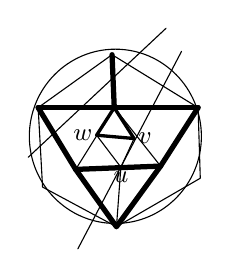
\begin{tikzpicture}[x=0.014cm,y=-0.014cm,line cap=round,line join=round,font=\small]
\coordinate (A) at (76,24);
\coordinate (B) at (9,72);
\coordinate (C) at (154,72);
\coordinate (D) at (80,180);
\coordinate (E) at (13,144);
\coordinate (F) at (156,136);
\coordinate (T) at (78,72);
\coordinate (U) at (43,128);
\coordinate (V) at (120,125);
\coordinate (W) at (62,97);
\coordinate (X) at (96,100);
\coordinate (Y) at (84,126);
\coordinate (L) at (125,0);
\coordinate (R) at (0,117);
\coordinate (J) at (139,21);
\coordinate (K) at (45,200);
\draw (A)--(B)--(E)--(D)--(F)--(C)--cycle;
\draw[line width=1.9pt] (B)--(T)--(C);
\draw[line width=1.9pt] (B)--(U)--(D)--(V)--(C);
\draw[line width=1.9pt] (U)--(V);
\draw[line width=1.9pt] (A)--(T);
\draw[very thick] (T)--(W)--(X)--cycle;
\draw (W)--(Y)--(X);
\draw (T)--(U);
\draw (T)--(V);
\draw (Y)--(D);
\draw[thin] (L)--(R);
\draw[thin] (J)--(K);
\node[left,inner sep=1.3pt] at (W) {$\unsure{w}$};
\node[right,inner sep=1.3pt] at (X) {$v$};
\node[below,inner sep=1.3pt] at (Y) {$u$};
\draw (79,98) ellipse[x radius=78,y radius=79];
\end{tikzpicture}}

\[
 S=T\amalg T_1\amalg T'_1\amalg T'_{\deleted{\unsure{1|2}}}
\]

\diagram{\begin{tikzcd}[ampersand replacement=\&,column sep=small,row sep=large,execute at end picture={\draw (topT.north west) rectangle (topPrime.south east); \path (topT.north) -- node[above] {$t\mapsto t'$} (topPrime.north);}]
t\arrow[d]\& |[alias=topT]| T\arrow[r,"\sim" description]\arrow[d,phantom,"\simeq" description]\& |[alias=topPrime]| T'\arrow[d,phantom,"\simeq" description]\&t'\arrow[d]\\
t_1\&T_1\arrow[r,"\sim","{t_1\mapsto t'_1}"']\&T'_1\&t'_1
\end{tikzcd}}

\deleted{\unsure{triangles}} couple de 2 triangles en corr 1-1

($B_3$)
\figure{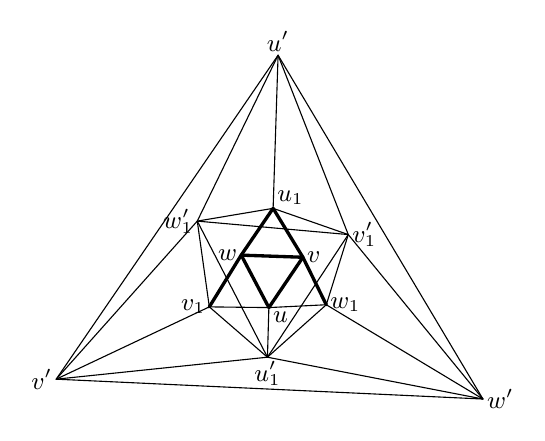
\begin{tikzpicture}[x=0.009cm,y=-0.009cm,line cap=round,line join=round,font=\small]
\coordinate (A) at (313,0);
\coordinate (B) at (0,457);
\coordinate (C) at (602,485);
\coordinate (M) at (199,234);
\coordinate (N) at (412,253);
\coordinate (P) at (298,426);
\coordinate (A1) at (306,216);
\coordinate (B1) at (216,355);
\coordinate (C1) at (381,352);
\coordinate (U) at (300,356);
\coordinate (V) at (348,285);
\coordinate (W) at (261,282);
\draw (A)--(B)--(C)--cycle;
\draw (A)--(M)--(B);
\draw (A)--(N)--(C);
\draw (B)--(P)--(C);
\draw (A)--(A1);
\draw (B)--(B1);
\draw (C)--(C1);
\draw (M)--(N)--(P)--cycle;
\draw (M)--(A1)--(N)--(C1)--(P)--(B1)--cycle;
\draw[very thick] (A1)--(W)--(U)--(V)--cycle;
\draw[very thick] (B1)--(W)--(V)--(C1);
\draw (B1)--(U)--(C1);
\draw (P)--(U);
\node[above,inner sep=1.3pt] at (A) {$u'$};
\node[left,inner sep=1.3pt] at (B) {$v'$};
\node[right,inner sep=1.3pt] at (C) {$w'$};
\node[left,inner sep=1.3pt] at (M) {$w'_1$};
\node[right,inner sep=1.3pt] at (N) {$v'_1$};
\node[below,inner sep=1.3pt] at (P) {$u'_1$};
\node[above right,inner sep=1.3pt] at (A1) {$u_1$};
\node[left,inner sep=1.3pt] at (B1) {$v_1$};
\node[right,inner sep=1.3pt] at (C1) {$w_1$};
\node[below right,inner sep=1.3pt] at (U) {$u$};
\node[right,inner sep=1.3pt] at (V) {$v$};
\node[left,inner sep=1.3pt] at (W) {$w$};
\end{tikzpicture}}

\diagram{$A\ \text{(arêtes)}\quad
\begin{array}{lll}
 \bigl\{\ \mathfrak P_2(T)&\mathfrak P_2(T')&6\\
 \left\{\begin{array}{c}\{\underset{\substack{\rotatebox{-90}{$\in$}\\T}}{t},\underset{\substack{\rotatebox{-90}{$\in$}\\T_1}}{u}\}\\u\ne t_1\end{array}\right.&
 \begin{array}{c}\{\underset{\substack{\rotatebox{-90}{$\in$}\\T'}}{t'},\underset{\substack{\rotatebox{-90}{$\in$}\\T'_1}}{u'}\}\\u'\ne t'_1\end{array}&12\\
 \left\{\begin{array}{c}\{\underset{\substack{\rotatebox{-90}{$\in$}\\T_1}}{\unsure{t|t_1}},\underset{\substack{\rotatebox{-90}{$\in$}\\T'_1}}{u}\}\\u\ne t'\end{array}\right.&&6\\
 \bigl\{\ \{t,t'_1\},\ \{t',t_1\}&&6
\end{array}$}

(C)

($C_1$)
\figure{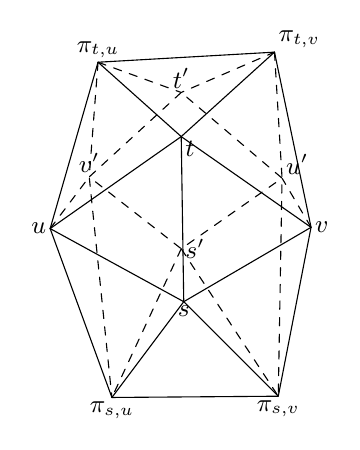
\begin{tikzpicture}[x=0.016cm,y=-0.016cm,line cap=round,line join=round,font=\small]
\coordinate (NW) at (38,8);
\coordinate (NE) at (178,0);
\coordinate (SW) at (49,274);
\coordinate (SE) at (181,273);
\coordinate (L) at (0,140);
\coordinate (R) at (207,139);
\coordinate (T) at (104,67);
\coordinate (S) at (106,198);
\coordinate (Tp) at (104,32);
\coordinate (Sp) at (104,156);
\coordinate (Lp) at (31,99);
\coordinate (Rp) at (184,100);
\draw (NW)--(NE)--(R)--(SE)--(SW)--(L)--cycle;
\draw (NW)--(T)--(NE);
\draw (L)--(T)--(R);
\draw (L)--(S)--(R);
\draw (T)--(S);
\draw (SW)--(S)--(SE);
\draw[dashed] (NW)--(Lp)--(SW);
\draw[dashed] (NE)--(Rp)--(SE);
\draw[dashed] (NW)--(Tp)--(NE);
\draw[dashed] (Tp)--(Lp)--(Sp)--(Rp)--cycle;
\draw[dashed] (Sp)--(SW);
\draw[dashed] (Sp)--(SE);
\draw[dashed] (L)--(Lp);
\draw[dashed] (R)--(Rp);
\node[above,inner sep=1.3pt] at (NW) {$\pi_{t,u}$};
\node[above right,inner sep=1.3pt] at (NE) {$\pi_{t,v}$};
\node[below,inner sep=1.3pt] at (SW) {$\pi_{s,u}$};
\node[below,inner sep=1.3pt] at (SE) {$\pi_{s,v}$};
\node[left,inner sep=1.3pt] at (L) {$u$};
\node[right,inner sep=1.3pt] at (R) {$v$};
\node[below right,inner sep=1.3pt] at (T) {$t$};
\node[below,inner sep=1.3pt] at (S) {$s$};
\node[above,inner sep=1.3pt] at (Tp) {$t'$};
\node[right,inner sep=1.3pt] at (Sp) {$s'$};
\node[above,inner sep=1.3pt] at (Lp) {$v'$};
\node[above right,inner sep=1.3pt] at (Rp) {$u'$};
\end{tikzpicture}}

ou

($C_2$)
\figure{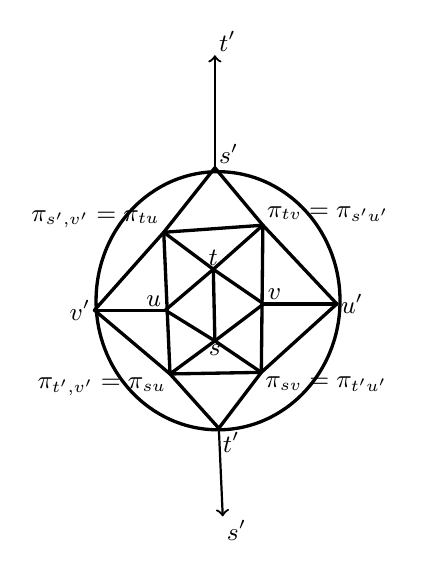
\begin{tikzpicture}[x=0.01cm,y=-0.01cm,line cap=round,line join=round,font=\small]
\coordinate (T) at (153,143);
\coordinate (B) at (158,474);
\coordinate (L) at (0,324);
\coordinate (R) at (308,316);
\coordinate (Nu) at (88,225);
\coordinate (Nv) at (214,216);
\coordinate (Su) at (96,405);
\coordinate (Sv) at (212,403);
\coordinate (U) at (90,324);
\coordinate (V) at (215,316);
\coordinate (Tt) at (151,272);
\coordinate (St) at (153,363);
\coordinate (E) at (153,0);
\coordinate (D) at (163,586);
\draw[very thick] (T)--(Nu)--(L)--(Su)--(B)--(Sv)--(R)--(Nv)--cycle;
\draw[very thick] (Nu)--(Nv)--(Sv)--(Su)--cycle;
\draw[very thick] (U)--(Tt)--(V)--(St)--cycle;
\draw[very thick] (Tt)--(St);
\draw[very thick] (U)--(L);
\draw[very thick] (V)--(R);
\draw[very thick] (Nu)--(Tt)--(Nv);
\draw[very thick] (Su)--(St)--(Sv);
\draw[->,thick] (T)--(E);
\draw[->,thick] (B)--(D);
\node[above right,inner sep=1.3pt] at (T) {$s'$};
\node[below right,inner sep=1.3pt] at (B) {$t'$};
\node[left,inner sep=1.3pt] at (L) {$v'$};
\node[right,inner sep=1.3pt] at (R) {$u'$};
\node[above left,inner sep=1.3pt] at (U) {$u$};
\node[above right,inner sep=1.3pt] at (V) {$v$};
\node[below,inner sep=1.3pt] at (St) {$s$};
\node[above,inner sep=1.3pt] at (Tt) {$t$};
\node[above left,inner sep=1.3pt] at (Nu) {$\pi_{s',v'}=\pi_{tu}$};
\node[above right,inner sep=1.3pt] at (Nv) {$\pi_{tv}=\pi_{s'u'}$};
\node[below left,inner sep=1.3pt] at (Su) {$\pi_{t',v'}=\pi_{su}$};
\node[below right,inner sep=1.3pt] at (Sv) {$\pi_{sv}=\pi_{t'u'}$};
\node[above right,inner sep=1.3pt] at (E) {$t'$};
\node[below right,inner sep=1.3pt] at (D) {$s'$};
\draw[very thick] (157,312) ellipse[x radius=155,y radius=164];
\end{tikzpicture}}

($C_3$)
\figure{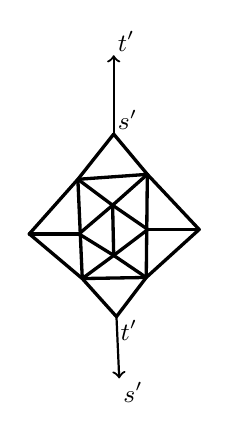
\begin{tikzpicture}[x=0.007cm,y=-0.007cm,line cap=round,line join=round,font=\small]
\coordinate (T) at (153,143);
\coordinate (B) at (158,474);
\coordinate (L) at (0,324);
\coordinate (R) at (308,316);
\coordinate (Nu) at (88,225);
\coordinate (Nv) at (214,216);
\coordinate (Su) at (96,405);
\coordinate (Sv) at (212,403);
\coordinate (U) at (90,324);
\coordinate (V) at (215,316);
\coordinate (Tt) at (151,272);
\coordinate (St) at (153,363);
\coordinate (E) at (153,0);
\coordinate (D) at (163,586);
\draw[very thick] (T)--(Nu)--(L)--(Su)--(B)--(Sv)--(R)--(Nv)--cycle;
\draw[very thick] (Nu)--(Nv)--(Sv)--(Su)--cycle;
\draw[very thick] (U)--(Tt)--(V)--(St)--cycle;
\draw[very thick] (Tt)--(St);
\draw[very thick] (U)--(L);
\draw[very thick] (V)--(R);
\draw[very thick] (Nu)--(Tt)--(Nv);
\draw[very thick] (Su)--(St)--(Sv);
\draw[->,thick] (T)--(E);
\draw[->,thick] (B)--(D);
\draw (T)--(Nv);
\draw (L)--(Nu);
\draw (R)--(Sv);
\draw (B)--(Su);
\node[above right,inner sep=1.3pt] at (T) {$s'$};
\node[below right,inner sep=1.3pt] at (B) {$t'$};
\node[above right,inner sep=1.3pt] at (E) {$t'$};
\node[below right,inner sep=1.3pt] at (D) {$s'$};
\end{tikzpicture}}

\uline{autom.} $\mathbb Z_2\times(\mathbb Z_2\times\mathbb Z_2)$ d'ordre $8=120/15$

\uline{NB} $15=30/2$

\[
 S=\unsure{\sigma|\underline{\sigma}}\amalg\varphi\amalg\sigma'\amalg\varphi'
 \amalg[\sigma\times\varphi\amalg\sigma'\times\varphi'\unsure{\}|/|\sim}]/\mathbb Z/2\mathbb Z
\]

\deleted{$(s,u)\unsure{\sim}(t',v')$ \unsure{si $s\ne t$,}} $\sigma$ opérant par

\[
 \sigma(s,u)=((\varepsilon s)',(\varepsilon u)')
\]

antipodisme \quad $a(s,u)=(\varepsilon s,\varepsilon u)$

\deleted{\unsure{$a$}} $(s,u)\in a\times b$ ou $(s,u)\in(a'\times b')$

\diagram{\begin{tikzpicture}[baseline=(edgeTable.base)]
\node[inner sep=2pt] (edgeTable) {$A:\left|\begin{array}{lll}
 \sigma,\sigma'&\deleted{4}&2\\
 \{\underset{\substack{\rotatebox{-90}{$\in$}\\\sigma}}{s},\underset{\substack{\rotatebox{-90}{$\in$}\\\varphi}}{u}\},\ \{\underset{\substack{\rotatebox{-90}{$\in$}\\\sigma'}}{s'},\underset{\substack{\rotatebox{-90}{$\in$}\\\varphi'}}{u'}\}&&8\\
 \{\pi_{s,u},\pi_{t,v}\}\quad\unsure{u|w}\ 
 \deleted{\unsure{(s,t)}}\ u\ne v &\deleted{\unsure{2|4}}&2\\
 \multicolumn{3}{l}{\hspace{2em}\sigma\quad\varphi\quad\varphi\quad\deleted{\unsure{s,t\ne}}}\\
 \{u,\pi_{s,u}\},\ \{u',\pi_{s',u'}\}&&8\\
 \{s,\pi_{s,u}\},\ \{s',\pi_{s',u'}\}&&8
\end{array}\right.$};
\path (edgeTable.south west) -- coordinate[pos=.56] (ringLeft) coordinate[pos=.84] (ringUpper) (edgeTable.north west);
\path (edgeTable.south east) -- coordinate[pos=.56] (ringRight) coordinate[pos=.84] (ringTopRight) (edgeTable.north east);
\draw (ringLeft) .. controls +(0,-.20) and +(0,-.15) .. (ringRight) .. controls +(.35,0) and +(.35,0) .. (ringTopRight) .. controls +(0,.12) and +(0,.15) .. (ringUpper) .. controls +(-.2,0) and +(-.2,0) .. (ringLeft);
\path (edgeTable.south west) -- coordinate[pos=.43] (leadersEnd) (edgeTable.north west);
\draw[->] (ringLeft) .. controls +(-.38,-.15) and +(-.18,0) .. (leadersEnd);
\end{tikzpicture}}

\[
 \boxed{\{u{},v'\},\ u\ne v\qquad 2}
\]

% archive sheet number: 8

